
\begin{slide}{Umfeld: Projekt L�ufer}
\begin{itemize}
  \item Studentisches Projekt
  \item Interdisziplin�res Team
  \item Alternative Form des Studiums
  \item Entwicklung eines ,,muskelgetriebenen Reisefahrzeugs''
  \item Industriepartnerschaften
  \item Innovative Technologien
\end{itemize}
\end{slide}


% ============================================================


\overlays{4}{%
  \begin{slide}{Aufgabe dieser Arbeit}
    \begin{center}
      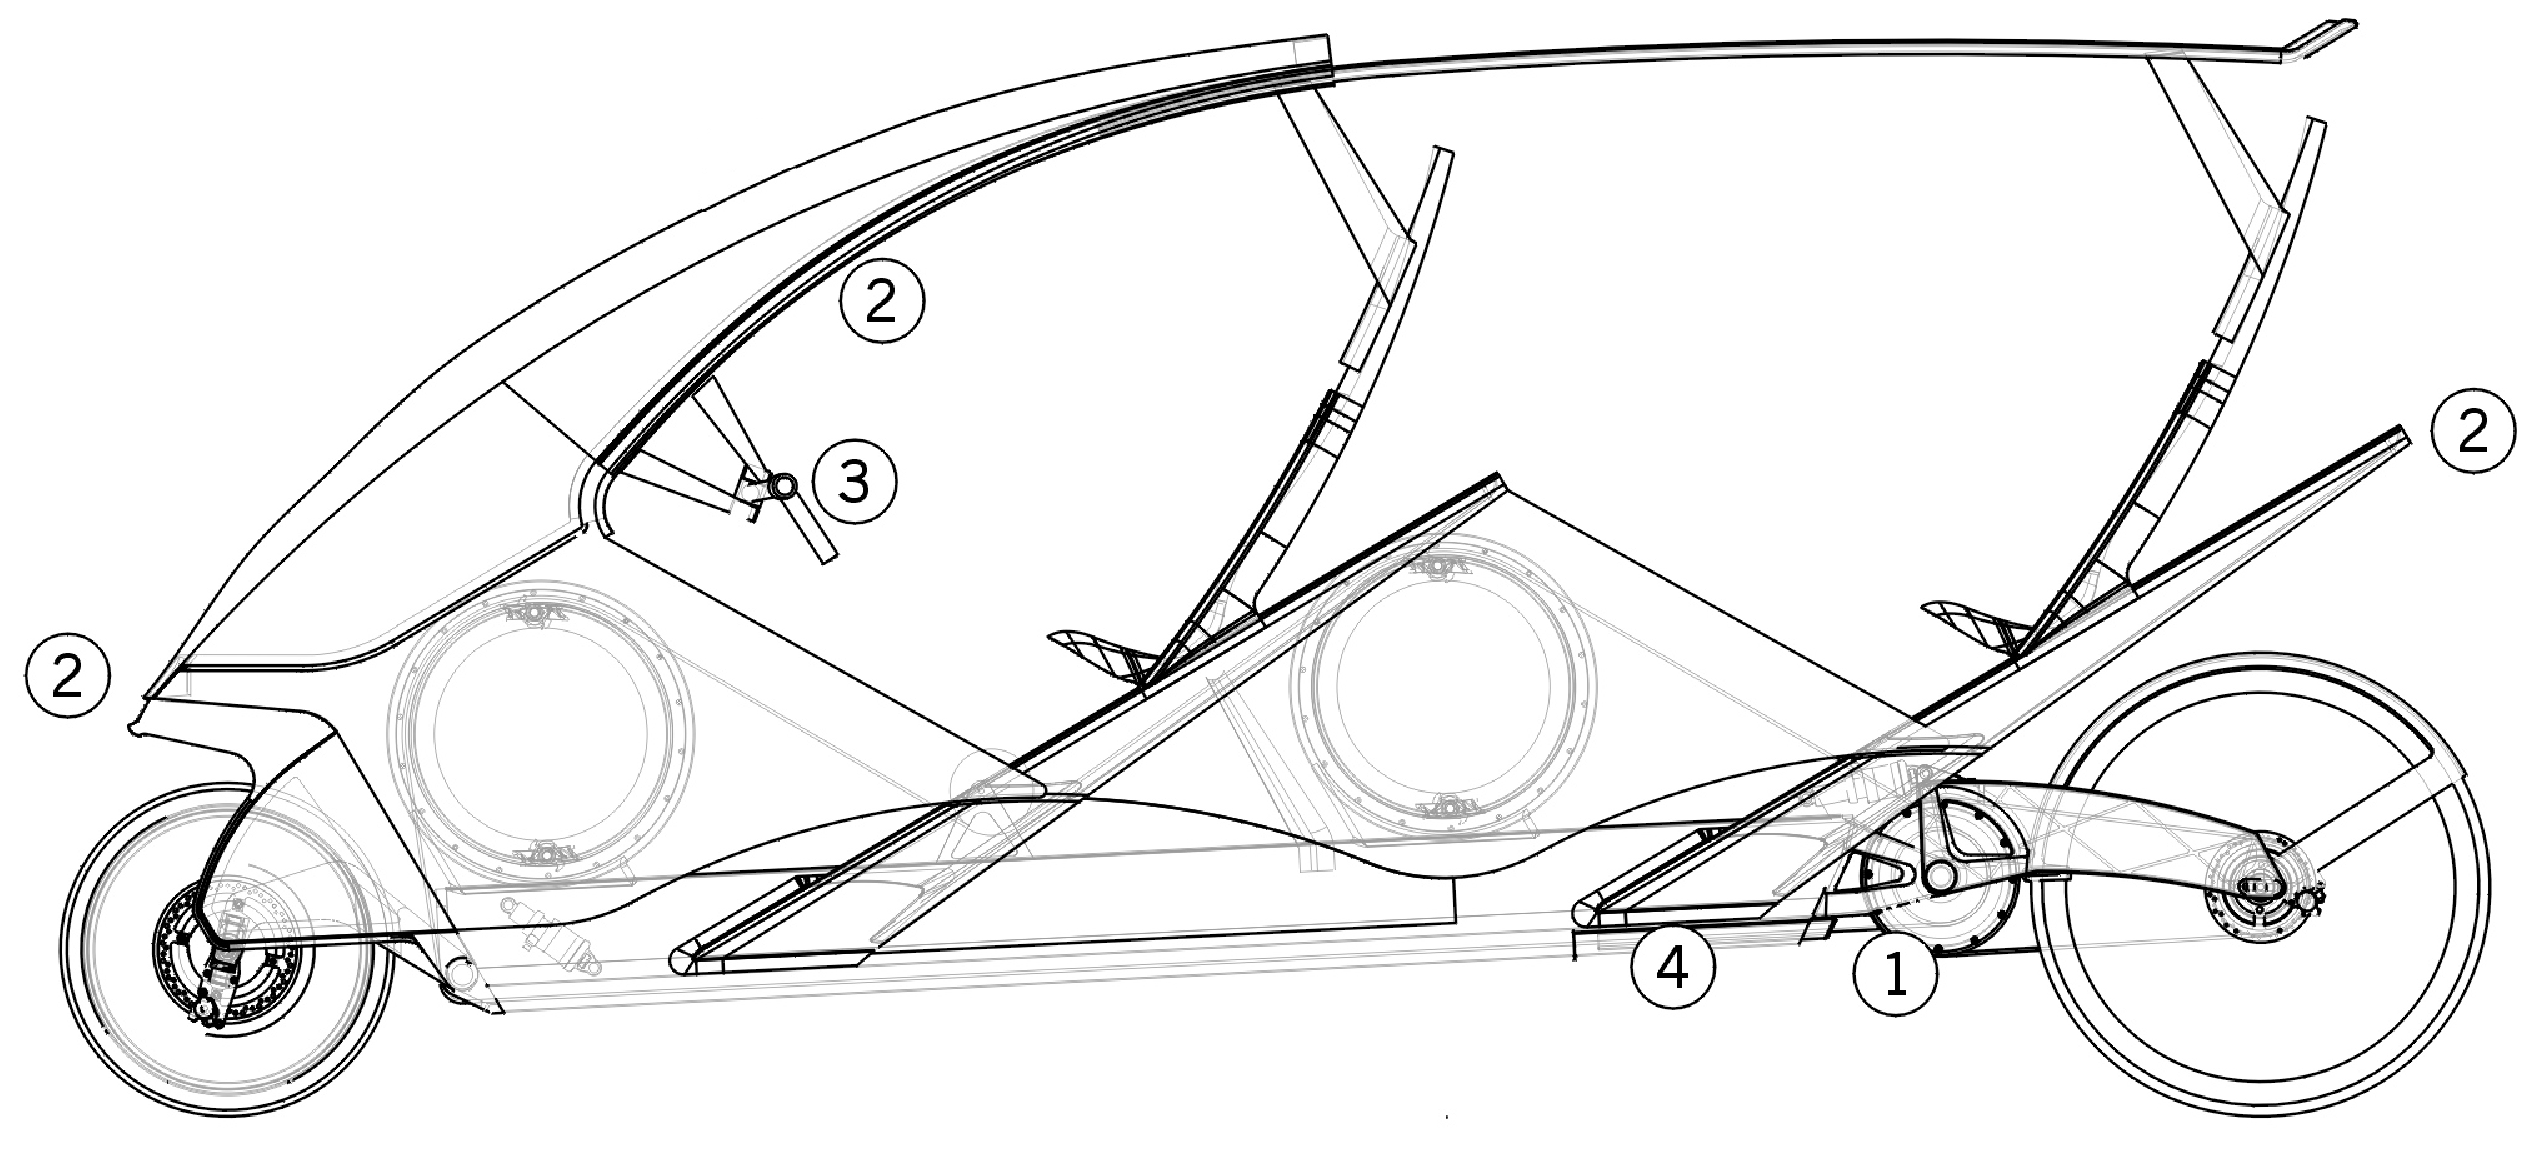
\includegraphics[width=10cm]{laeufer.eps}
      \onlySlide*{1}{Entwicklung eines Mechatronik-Frameworks}%
      \onlySlide*{2}{Platinen samt Mini-Betriebssystem (2)}%
      \onlySlide*{3}{Kommunikation (1-4)}%
      \onlySlide*{4}{Fahrer-Schnittstelle (3)}%
    \end{center}
  \end{slide}
}

% ============================================================


\begin{slide}{Ziele}
Das erstelle Mechatronik-Framework soll
\begin{itemize}
  \item sp�ter von den Ingenieuren handhabbar,
  \item durch Industriepartner f�rderbar,
  \item flexibel erweiterbar und
  \item funktionierend
\end{itemize}
sein.
\end{slide}


% ============================================================


\begin{slide}{�bersicht �ber das Folgende}
Weg eines Benutzerwunsches:
\begin{itemize}
  \item Benutzer dr�ckt Blinker-Knopf
  \item Weg durch den PDA und die Kommunikation
  \item Umsetzung des Benutzerwunsches auf der Platine
  \item Feststellung eines Fehlers samt Benachrichtigung des Fahrers
\end{itemize}
\end{slide}

